\subsection{ROTE}

To overcome the slowness of SGX Monotonic Counters and provide stable persistent 
rollback attack protections, ROTE~\cite{} is proposed as a distributed trusted 
counter service based on a consensus protocol.

\subsubsection{Overview of ROTE}
\label{overview_rote}
ROTE is a \textit{inc-then-store} based system that protects against rollback attacks.
To overcome the low throughput of monotonic counter increment, ROTE uses a distributed 
secure counter storage to help verify the version of a target enclave. The intuition 
behind is simple, that a single SGX-enabled platform is difficult to prevent rollback
attacks but many platforms can work together to assist the process of verification.
The assisting servers are incentive to do this job as they can also benefit from 
such protection.

With the assistance of a group of servers, ROTE assumes a strong adversary  
that can either control the OS of the target platform or any of the assisting platforms.
The adversary can break the protection of SGX and even act as a network-level administrator
that controls the interactive communication in the network by delaying, replaying or 
revising network packets. However, as a \textit{inc-then-store} based system, ROTE 
assumes no tolerance of some of the platform crashes and by default no crash will happen
in a protocol run. If crash tolerance is required, then a \textit{store-then-inc}
technique is required, and even the system should support both of the techniques to 
allow users choose by their tolerance of crash.

The update stage of ROTE works as follows. A client first triggers a counter increment 
in local enclave, the enclave increments the counter (initialized as zero) in runtime
memory, signs the counter value and sends the signed counter value to all assisting 
servers. Upon receiving the signed counter value, each assisting server updates the 
value of targeting (client's) counter table in memory and sends back their state 
of counter value. Note that the value is temporarily stored in memory 
and not sealed to disk to avoid endless propagation. When the client receives $q$
feedbacks, it compares the value and returns ACks if the value matches its own.
Then, the client can ensure that the version is correct, seal the current counter 
value and the object to disk. 

ROTE also develops a protocol to recover from system reboot/failure, and a distributed 
mechanism to securely store and compare counter values in remote assisting servers.
With a strong network adversary model, ROTE protects
against both network partitioning and replay attacks. The update protocol, 
recover protocol and distributed secure storage mechanism work together to make ROTE 
a robust KVS system that provides protection against rollback attacks.



\subsubsection{System Protocols}
\begin{figure}
    \centering
        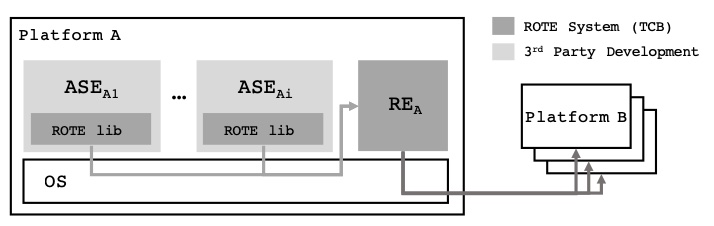
\includegraphics[width=.45\textwidth]{rote_sys}
        \caption[title]{The ROTE system architecture.}
        \label{fig:rote_sys}
\end{figure}

Figure \ref{fig:rote_sys} shows ROTE system architecture. Every user application running on platforms matches an Application-Specific Enclave (ASE). The ROTE system provides a Rollback Enclave (RE) and a ROTE library for ASEs as a rollback protection service. The RE maintains a Monotonic Counter (MC), increases it for every ASE update, distributes it to REs running on assisting platforms, and includes the counter value to its own sealed data. 

For easier descriptions, we denote $n$ as the number of assisting platforms, $f$ as the number of compromised processors, and $u$ as the tolerance of  unreachable assisting platforms when the system proceeds write/read operation. These three parameters have a dependency $n = f + 2u + 1$ to fulfill the data integrity, attestation and freshness of the ROTE system consensus protocols. In the ROTE system, there are three protocols designed for ASE state update, RE restart, and ASE start/read. Specifically, messages transmitted in the ROTE system are all encrypted with respective session keys for data confidentiality concerns. We respectively specify them as follows.
\begin{itemize}
	\item \textbf{ASE State Update Protocol} When an ASE is ready to update its state, it starts the state update protocol. This protocol can be regarded as a modification of the Echo broadcast~\cite{}. 
	\begin{enumerate}
		\item The ASE triggers a counter increment using the RE.
		\item The RE increments its own MC, and signs the MC. 
		\item The RE sends the signed counter to all REs in the protection group.
		\item Upon receiving the signed MC, each RE updates its group counter table kept in the runtime memory without sealing the received data.
		\item The REs that received the counter saves the echo in runtime memory and broadcasts an echo message containing the received signed MC.
		\item After receiving $q=u+f+1$ echos, the RE returns the echos to their senders.
		\item Upon receiving back the echo, each RE finds the self-sent echo in its memory. Then every RE checks if the value from echo, from the group counter table, and from the target RE are equal. If these three values match each other, the RE replies with a final ACK message.
		\item After receiving $q=u+f+1$ final ACKs, the RE seals its own state together with the MC value to the disk.
		\item The RE returns the incremented ASE counter value. The ASE can now safely perform the state update. The ASE saves the counter value to its runtime memory and seal its state with the counter.
	\end{enumerate}
	\item \textbf{RE Restart Protocol} The goal of the protocol is to allow the RE to join the existing protection group, retrieve its counter value and the MC values of the other nodes. It supports at most $u$ REs restart simultaneously. 
	\begin{enumerate}
		\item Reset cryptology keys and update system configuration informations
		\item The RE queries the OS for the sealed state.
		\item The RE unseals the state (if received) and extracts the MC.
		\item \label{s}The RE sends a request to all other REs in the same protection group to retrieve its MC.
		\item The assisting REs check their group counter table. If the MC is found, the enclaves reply with the signed MC. Additionally, the target RE receives the complete table all signed MCs from assisting REs.
		\item \label{e}When the RE receives $q=u+f+1$, where $q \ge n/2$ with at least $f+1$ counter values not zero, responses from the group, it selects the maximum value and verifies the signature. For each assisting RE, the target RE picks the highest MC and updates its own group counter table with the value. If the obtained counter value equals to the unsealed data, the unsealed state can be accepted.
		\item The RE stores and seals the updated state to both persistent and runtime memory.
		\end{enumerate}
	\item \textbf{ASE Start/Read Protocol} When an ASE needs to verify the freshness of its state, it performs this protocol.
	\begin{enumerate}
		\item The ASE queries the OS for the sealed data.
		\item The ASE unseals the state (if received) and obtains a counter value from it.
		\item The ASE issues a request to the local RE to retrieve its latest ASE counter value.
		\item To verify the freshness of its runtime state, the RE performs the steps \ref{s}-\ref{e} from the RE Restart protocol, to obtain the latest MC from the network. If the obtained MC does not match the MC residing in the memory, the RE must abort and be restarted. If the values match, the current data is fresh and the RE can continue normal operation.
		\item If all verification checks are successful, the RE returns a value from the local ASE counter table.
		\item The ASE compares the received counter value to the one obtained from the sealed data.
	\end{enumerate}
\end{itemize} 

Notice that in ROTE system defines a required quorum with size $q=u+f+1$ for secure consensus. The reason behind $q$ value is that if the counter is successfully written to $q = f + u + 1$ nodes, there always exists at least $u + 1$ honest platforms in the group that have the latest counter value in the memory. Because counter reading requires the same number of responses, at least one correct counter value is obtained upon reading. If the quorum cannot be satisfied in either the state update protocol or any counter retrieval, ROTE turns to halt and try to perform the same operation again.







%\begin{figure}
%    \centering
%        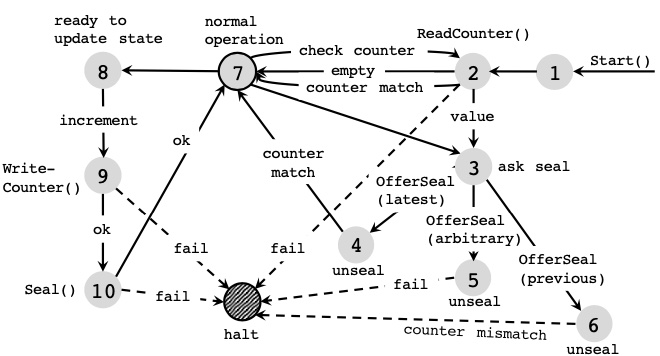
\includegraphics[width=.45\textwidth]{states}
%        \caption[title]{Transition diagram showing enclave execution states using an ideal secure counter storage functionality.}
%        \label{fig:states}
%\end{figure}


\subsubsection{Limitations}

As is mentioned above, ROTE leverages \textit{inc-then-store} counter increment 
technique as the foundation to defend against rollback attacks. The bottleneck 
of such technique still exists in ROTE: the crash during protocol run can totally 
ruin the system and prevent the system from recovery. 

We propose two future directions for further improving ROTE's trust model by enabling 
crash recovery between sealing counter values and sealing objects to disk.
Our first proposal is to ensure the atomicity of the \textit{write\_counter()} function
and \textit{seal\_object()} function. Currently in ROTE, the crash may happen between the 
two functions, contributing to a counter with a future value and making the KVS unrecoverable.
If we ensure the atomicity of the two functions, then the counter sealing and object sealing 
will succeed or fail at the same time, and the scenario where the counter has a future value 
will not appear.

Our second approach is to backup the counter value in disk, right before the verification 
of received counters in ROTE. In that case, if the crash happens after the sealing of counter
(before sealing the object), the KVS can still recover to the older version of counter value 
by referring to the log.
